 \documentclass[t]{beamer}
%\documentclass[c]{beamer}
\listfiles

\mode<presentation>
{
  \usetheme[english]{KIT}
% \usetheme[usefoot]{KIT}
% \usetheme{KIT}

%%  \usefonttheme{structurebold}

  \setbeamercovered{transparent}

  %\setbeamertemplate{enumerate items}[circle]
  \setbeamertemplate{enumerate items}[ball]

}
\usepackage{babel}
\date{23.09.2015}
%\DateText

\usepackage[latin1, utf8]{inputenc}
\usepackage[TS1,T1]{fontenc}
\usepackage{array}
\usepackage{multicol}
\usepackage{lipsum}
\usepackage{graphicx}
\usepackage{svg}
\usepackage{todonotes}

\usenavigationsymbols
%\usenavigationsymbols[sfHhdb]
%\usenavigationsymbols[sfhHb]

\title{Traffic Lane Detection in Urban Environments}
%\subtitle{Karlsruhe Institute of Technology (KIT)}

\author{Marin Vlastelica Pogančić}

%\AuthorTitleSep{\relax}

\institute[]{Forschüngszentrum Informatik (FZI)}


\TitleImage[width=\titleimagewd]{Bilder/KIT-Titel}

\newlength{\tmplen}

\newcommand{\verysmall}{\fontsize{6pt}{8.6pt}\selectfont}
\newcommand{\spank}{\setlength{\itemsep}{14pt}}


\begin{document}

\frame
{
  \maketitle
}

\frame
{
	\frametitle{Table of contents}
	\tableofcontents
}

\section{Motivation}

\frame
{
	\frametitle{Why Urban?}
	\begin{itemize}
		\spank
		\item Cluttered scenery challenging detection
		\item Unmarked streets
		\item Street signs
	\end{itemize}

	\missingfigure[figwidth=6cm]{Cluttered environment}
}

\frame
{
	\frametitle{Problems to be solved}
	\itemize
	{
		\spank
		\item Object detection -
		\item Trajectory estimation -
		\item Traffic sign detection -
		\item Lane marking detection +
		\item Curb detection +
		\item ...
	}
}

\section{Lane and curb detection requirements}

\frame
{
	\tableofcontents[ 
    currentsubsection, 
    sectionstyle=show/hide, 
    subsectionstyle=show/shaded,
    sectionstyle=show/shaded 
    ] 
}

\frame
{
	\frametitle{Commonly used sensors}
	\itemize
	{
		\spank
		\item 3D LADAR laser sensor
		\item Stereo camera
		\item Additional sensors for positioning and ego-motion estimation
		\
	}	
}


\section{Lane marking detection approaches}

\frame
{
	\frametitle{Table of contents}
	\tableofcontents[ 
    currentsubsection, 
    sectionstyle=show/hide, 
    subsectionstyle=show/shaded,
    sectionstyle=show/shaded 
    ] 
}

\frame
{
	\frametitle{Improved RANSAC algorithm}
	\itemize
	{
		\item RANSAC - the most common used algorithm\\
		for lane marking detection
		\item Used features: edges detected by the\\
		Canny detection algorithm
		\item Modeling lane markings with generalized curves
		\item Thereafter iterative estimation of the parameters
		\item Advantage: The RANSAC algorithm can adapt to the complex\\ conditions of lane estimation
of model parameters and it does not need training process
	}

	\begin{equation}
	x = \frac{a}{y-vp_y}+b(y-vp_y) +c
	\label{eq1}
	\end{equation}
}



\frame
{
	\frametitle{Improved RANSAC algorithm}
	TODO: ALGORITHM
}

\frame
{
	\frametitle{Improved RANSAC algorithm}
	\begin{figure}[ht]
	\centering
   	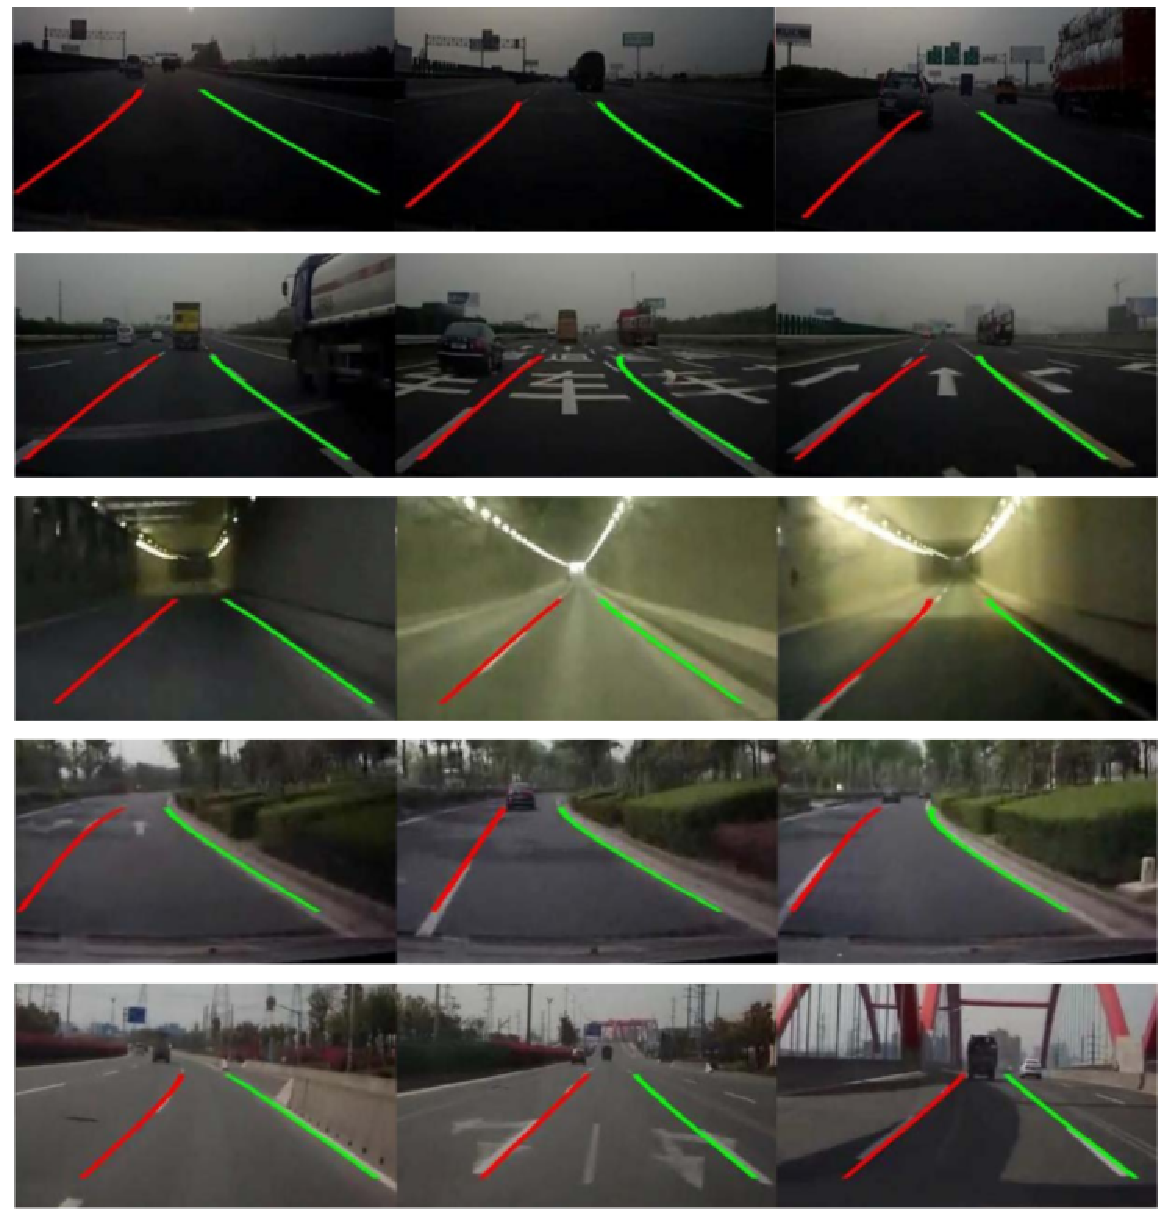
\includegraphics[scale = 0.3]{pictures/good_detections.pdf}
	\caption{Good detection results}
	\label{fig5}
	\end{figure}
}

\frame
{
	\frametitle{Improved RANSAC algorithm}
	\begin{figure}[ht]
	\centering
   	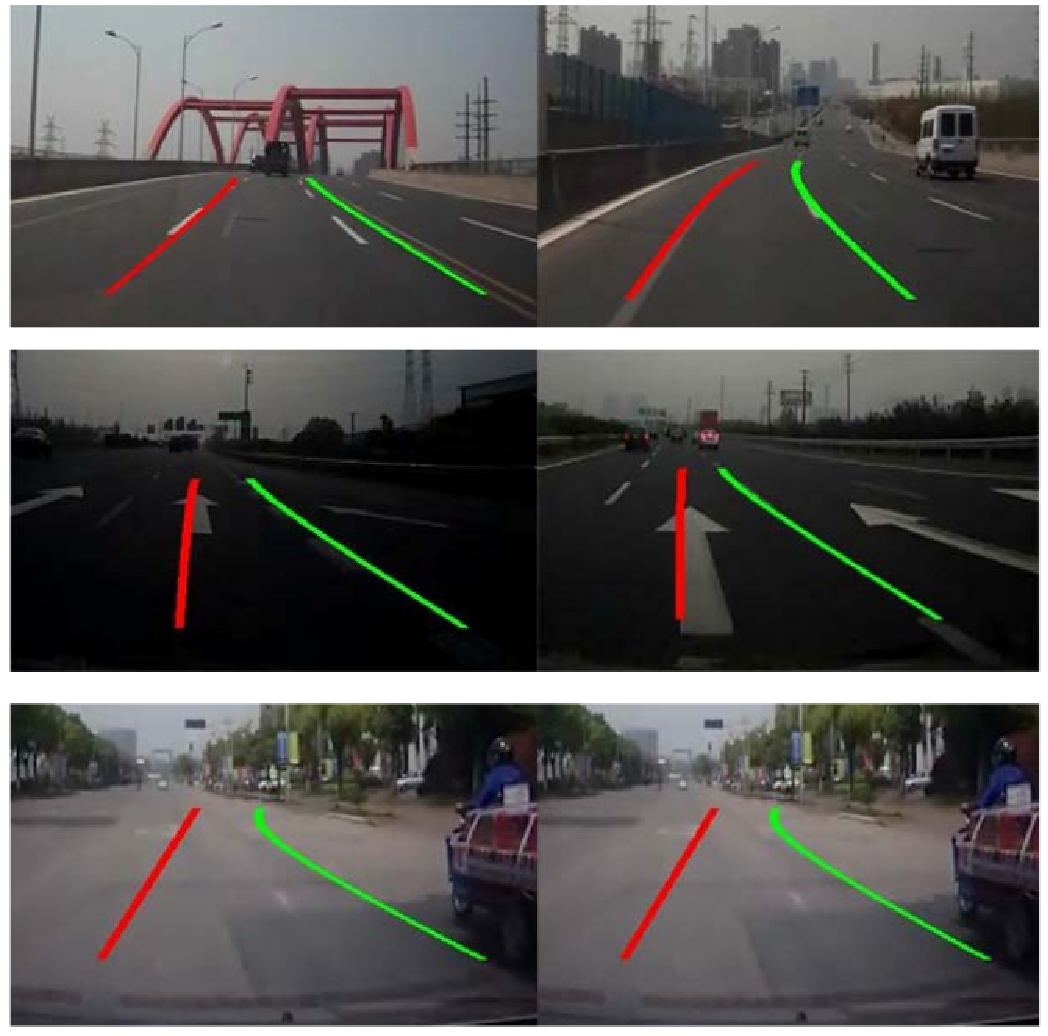
\includegraphics[scale = 0.3]{pictures/bad_detections.pdf}
	\caption{Bad detection results}
	\label{fig5}
	\end{figure}
}


\frame
{
	\frametitle{Tree based graphical model for lane detection}
	\itemize
	{
		\item Goal:  capture the way the joint distributions over \\random variables can be decomposed into a product of factors
		\item After the tree is generated, search tree with a search strategy
		\item Shortcoming: assume a flat road surface
	}

}

\frame
{
	\frametitle{Tree based graphical model for lane detection}


	\begin{figure}
	\centering
    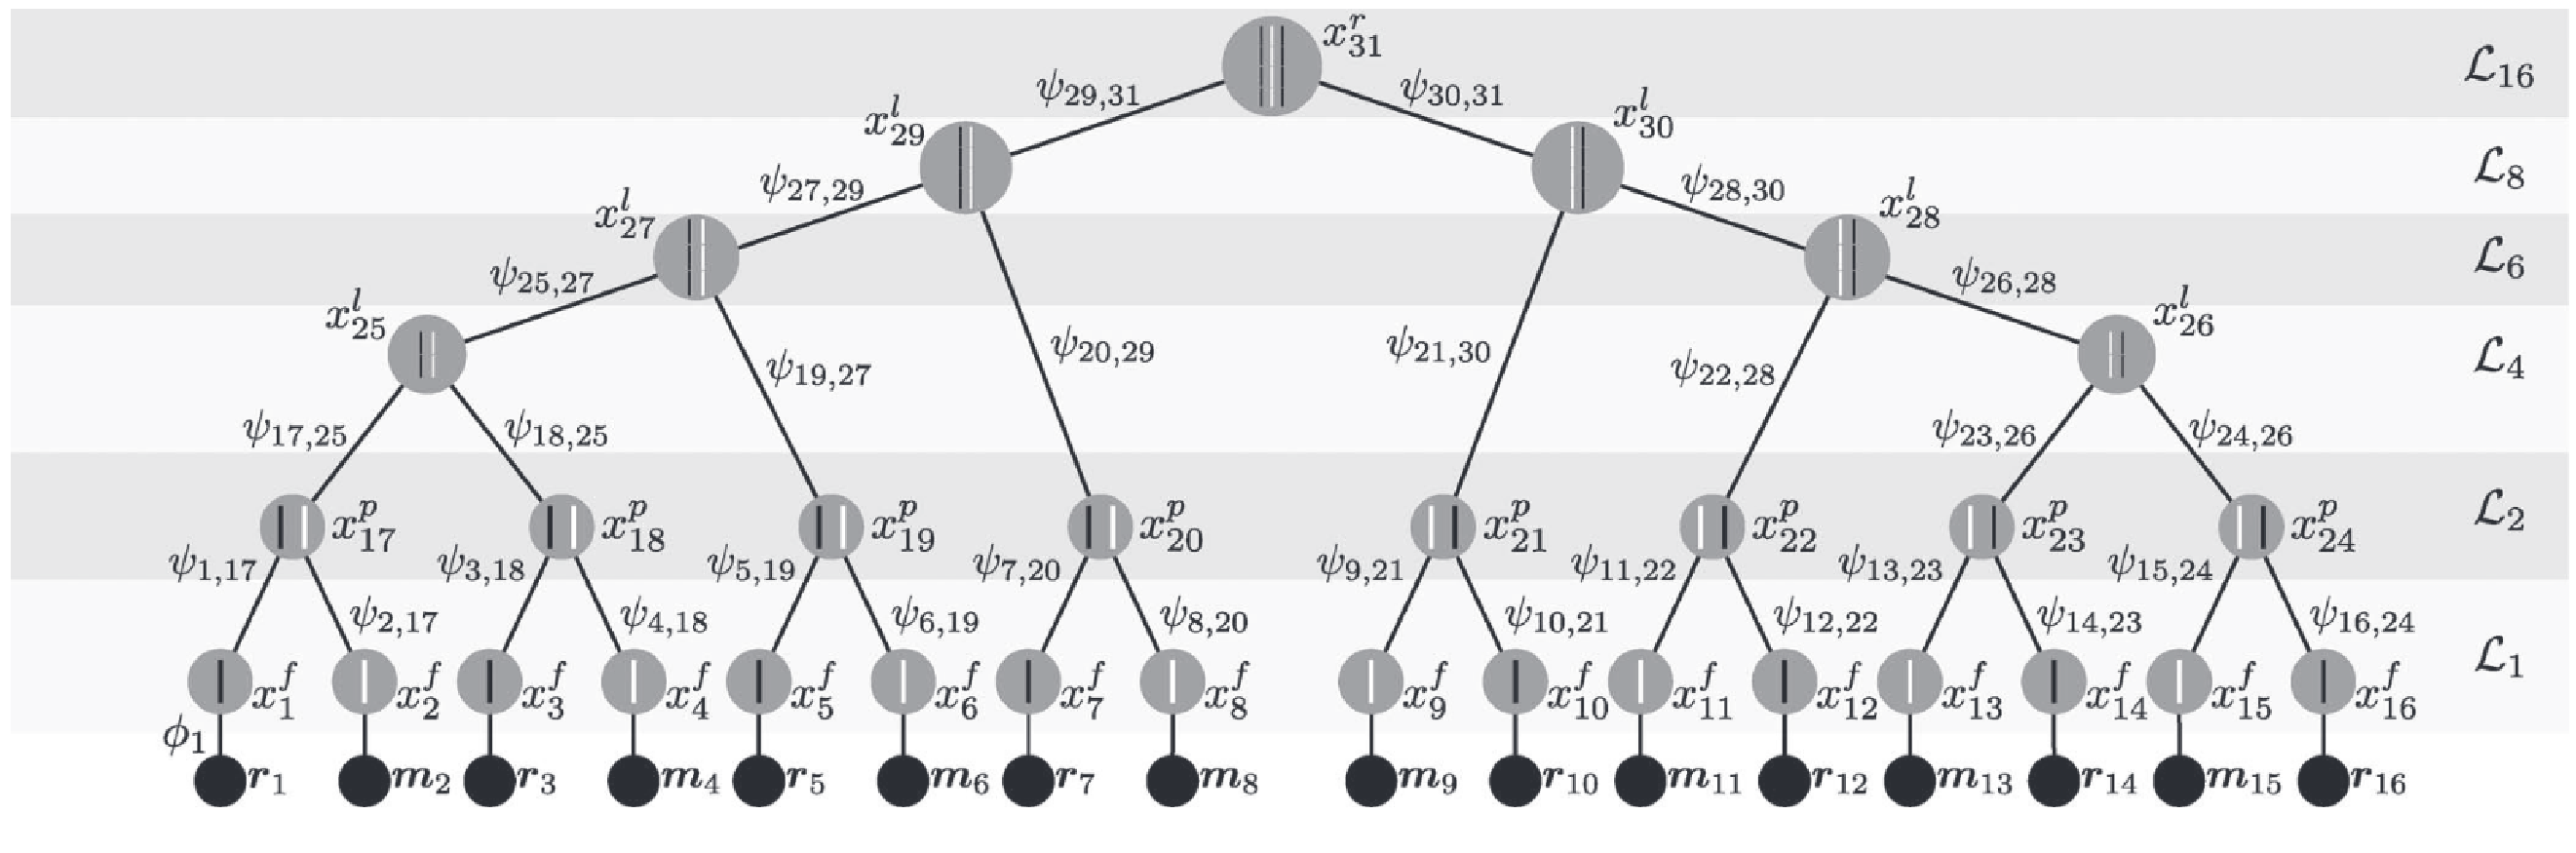
\includegraphics[scale = 0.25]{pictures/tree.pdf}
	\caption{CHM of a two-lane road. This figure shows the factorization of the joint probability distribution in (2) using an undirected graphical model. Hidden random variables are depicted in gray and symbols illustrate their type, i.e., features, patches, lanes, and multilane roads. Observable variables are shown in blackand dependencies between random variables are highlighted using edges.}
	\label{fig10}
	\end{figure}

}



\frame
{
	\frametitle{Tree based graphical model for lane detection}


	\begin{figure}[H]
	\centering
    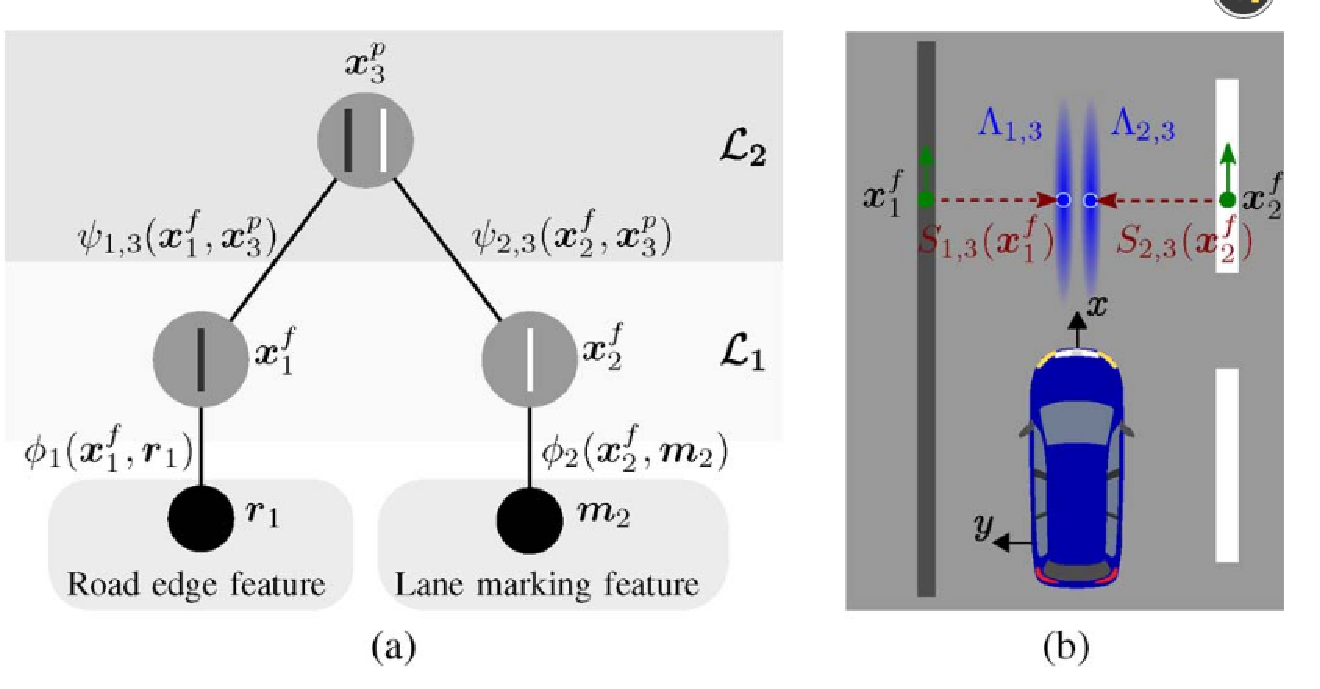
\includegraphics[scale = 0.25]{pictures/patch.pdf}
	\caption{CHM of a patch and illustration of the modeled spatial constraints, two tree leaves make a patch. (a) Patch is decomposed into a left and a right lane boundary, which are directly observable. (b) Illustration of the modeled spatial constraints, where spatial uncertainties are illustrated by showing 2-D Gaussian distributions, where dark colors correspond to more likely locations.}
	\label{fig11}
	\end{figure}

}



\section{Curb detection approaches}

\frame
{
	\frametitle{Table of contents}
	\tableofcontents[ 
    currentsubsection, 
    sectionstyle=show/hide, 
    subsectionstyle=show/shaded,
    sectionstyle=show/shaded 
    ] 
}

\frame
{
	\frametitle{Elevation mapping techniques with stereo camera}
	\itemize
	{
		\item Based on elevation maps
	}
	\enumerate
	{
		\item Generate point cloud from stereo camera
		\item Transform the point cloud from the sensor coordinate system to the map coordinate system
	}
}

\frame
{
	\frametitle{Different mapping techniques}

}


\frame
{
	\frametitle{Laserscanner based road curb detection}
}

\frame
{
	\frametitle{Laserscanner based road curb detection}

}

\section{Conclusion}

\frame
{
	\frametitle{Conclusion}
}

\section{Bibliograpgy}
\frame
{
	\frametitle{Bibliography}
}
\end{document}
